\subsection{Financial Markets}\label{subsec:assetprice}


% \begin{center}[Insert Figure \ref{fig:graph_investment}  here]\end{center}


\ifInBook{}{ % don't show these maps for book chapter
\begin{figure}[!ht] \centering  % [h!]
  \caption{ ~Literature map of EE models of stock/housing market investment}
  \label{fig:graph_investment}
  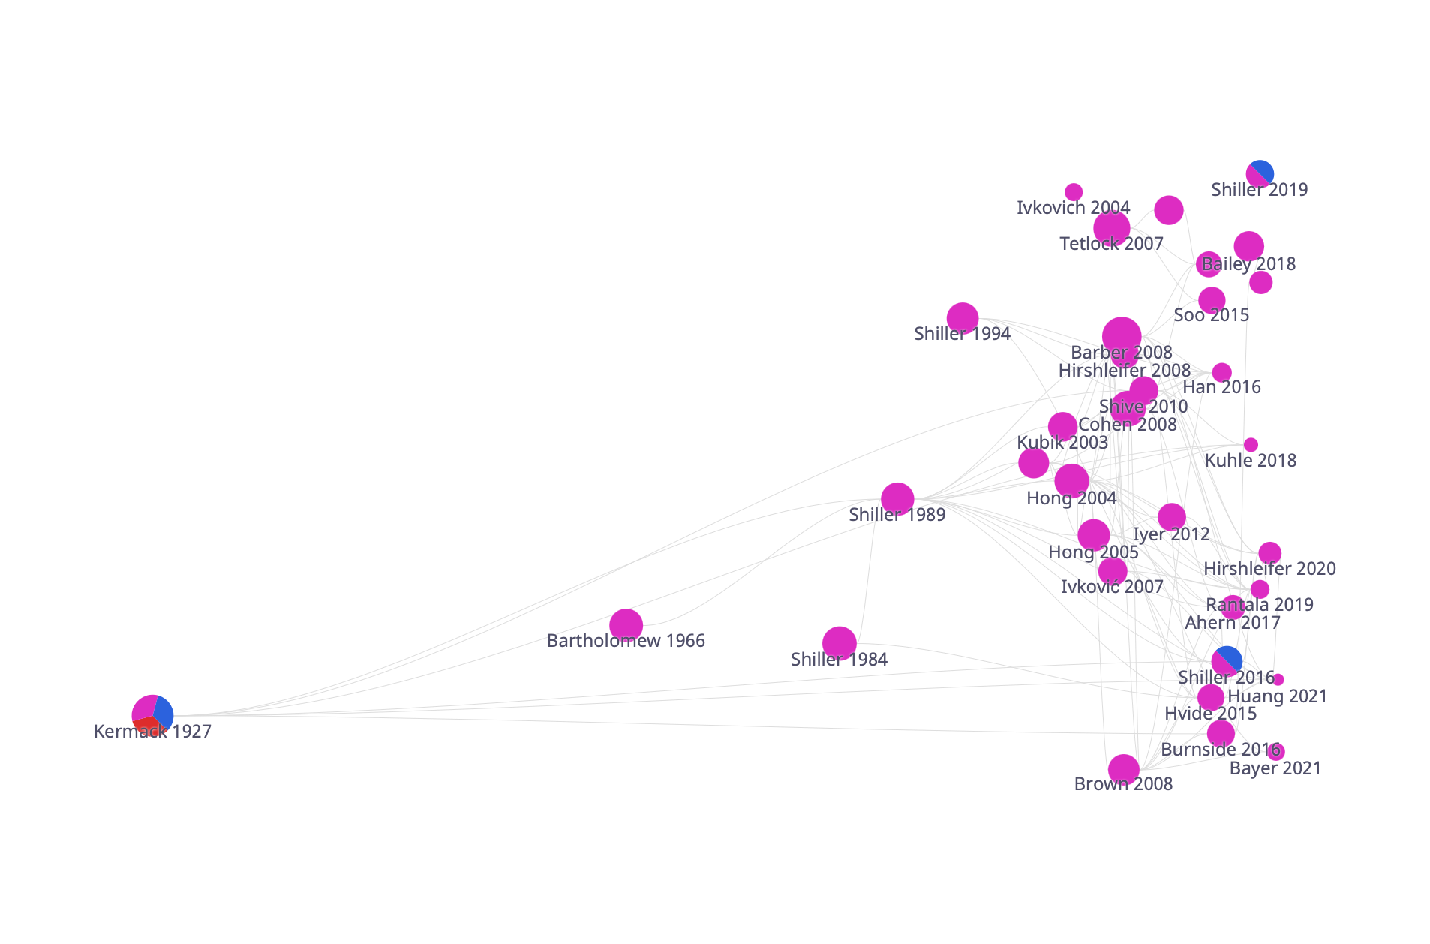
\includegraphics[width=\textwidth]{./figures/graph_investment.png}
  \begin{flushleft}
    {\footnotesize Note: This graph includes selected papers related to epidemiological models of expectations in asset markets, and studies of the role of news media in financial markets. See \href{https://app.litmaps.co/shared/E25276CA-8725-437B-8241-11961EFB3FB4}{here} for an interactive version.}
  \end{flushleft}
\end{figure}
}

Academic models of financial markets traditionally assume investors choose stocks based on self-generated rational beliefs about future returns.  But popular treatments have emphasized social communication, and ideas with a distinctly epidemiological flavor, since the first published description of  the first publicly traded securities (\cite{vegaConfusion}'s account of the trading of shares of the East India company on the Amsterdam stock exchange).  \cite{mackay_memoirs_1852}'s vivid prose has made his (thoroughly epidemiological) descriptions of the Dutch Tulip mania and other financial episodes of ``The Madness of Crowds'' a classic of English literature.  This popular emphasis on the importance of social interactions has continued to the present: Michael \cite{lewis2011big}'s bestseller about the financial crisis of 2008-09 goes so far as to suggest that one of the reasons a particular analyst was able to perceive the housing bubble early was his temperamental indifference to other people's opinions.

%% more excerpts: Abstract. I survey the advice given by the fifty most popular personal finance books and compare it to the prescriptions of normative academic economic models. Popular advice frequently departs from normative principles derived from economic theory, which should motivate new hypotheses about why households make the financial choices they do, as well as what financial choices households should make. I cover advice on asset allocation, savings rates, the advisability of being a wealthy hand-to-mouth consumer, non-mortgage debt management, simultaneous holding of high-interest debt and low-interest savings, and mortgage choices.

The academic tide seems now to be turning in this popular direction. \cite{hirshleifer2020presidential}'s Presidential Address to the American Finance Association urged the profession take up the study of the social transmission of ideas as ``[a] key but underexploited intellectual building block of social economics and finance,'' and argues that such models may be able to make sense of patterns that are difficult to understand with traditional models.  \cite{akccay2021social} make a broad argument that there are important biases in the transmission of ideas from one person to another which `shape market outcomes.' \cite{hirshleifer2015behavioral}, \cite{hirshleifer2020presidential} and \cite{kuchler2021social} propose `social finance' as the name for a field that would study the role of social interactions, and argue that new data and new methods could advance the field quickly.

These are by no means the first academics to propose a role for social transmission of financial ideas.  But the proportion of efforts that could be described as constituting a full-fledged EE analysis, as opposed to piecemeal evidence or provocative theoretical exercises, is small. % (See Figure \ref{fig:graph_investment})

An early example of such a comprehensive approach is  \cite{shiller1989survey}, used in Section~\ref{subsec:SIRModel} to delineate the elements of the generic SIR model.  Now we interpret its content as an economic model.  \cite{shiller1989survey} surveyed individual active investors to understand the sources of information that generated their initial interest in the stock they had most recently purchased (which they designate as `randomly selected' -- \texttt{RAND}), and in a set of stocks that have been ``rapidly rising.'' (`\texttt{RPI}').  Their separate survey of institutional investors used a different methodology to designate \texttt{RAND} and \texttt{RPI} stocks. %`rapidly rising' -- `\texttt{RPI}' -- stocks for institutional investors, they find that 10 percent and 30 percent of their initial interest originated from `nonprofessionals.'

Their survey-based estimates of the epidemiological parameters for both individual (`\texttt{IND}') and institutional (`\texttt{INS}') investors indicate considerable heterogeneity in infection rates both within and between the groups. The estimates also suggest that infectiousness differs between \texttt{RAND} and a \texttt{RPI} stocks. Interestingly, the \texttt{RAND} category is more (interpersonally) ``infectious'' than the rapidly rising category; the authors speculate that public news sources will already have widely covered rapidly rising stocks, so that interpersonal communications are unnecessary to attract attention.

Figure \ref{fig:sir_simulate} shows compartmental dynamics under their median estimates (of infection and removal rates) for individual and for institutional investors, and for randomly selected versus rising stocks, respectively.

The epidemiological parameters are estimated from a sample of highly interested and motivated investors -- which is why it is not surprising that all parameterizations were ones in which $\Recovered$ (the proportion of investors who would eventually become interested in a stock) converges to a high value.

The results can now also be interpreted in temporal terms.  The authors note that a fully rational model with no private information would imply that spikes in trading volume should immediately follow news events, while the epidemiological model is consistent with long and variable lags.  It takes around half a year for the interest of institutional investors in the randomly selected stocks to reach its peak and a little more than a year for a rapidly rising stock. For individual investors, the population interested in \texttt{RAND} reaches its peak after 40 weeks, while interest in \texttt{RPI} takes 2.5 years to peak.

The paper also argues that in a special case where the infection rate is close to the removal rate, and the size of the pool of interested investors is driven by serially uncorrelated shocks, stock prices could follow a random walk, because the change in the level of `interest' would be nearly unforecastable.\footnote{\cite{shiller1984stock} elaborates on this logic by allowing the presence of both rational investors (``smart money'') and social-dynamics driven investors. The presence of unforecastable social dynamics undermines the conclusion that a random walk implies full rationality.} %This is another example of an economic consequence flowing from in-principle measurable aspects of the pattern of spread of an infection.

Remarkably little of the large literature citing \cite{shiller1989survey} has involved meaningful epidemiological modeling; most has either been nonstructurally empirical, or has used a modeling framework that cannot really be characterized as `epidemiological.'
A likely reason for this lack of followup is the nonexistence of direct data on either of the two key components of the model: beliefs (about, say, stock prices); and social connections.  \ifInBook{}{\cite{shiller1989survey} had to make heroic assumptions to quantify their model.  Few subsequent scholars have been willing to go so far in employing what might today be termed an `indirect inference' approach: ``Assuming the epidemiological model is right, let's calibrate it using its downstream implications for things we can observe.''} We have found only two subsequent papers that estimate parameters of a structural epidemiological model of stock investors using microdata.

\IfPrivate{\href{https://github.com/iworld1991/EpiExp/blob/master/Literature/shive2010epidemic.pdf}{\cite{shive2010epidemic}}}{\cite{shive2010epidemic}} uses an SI (`susceptible-infected') model to figure out how to construct a reduced-form empirical regressor that aims to capture social influences among investors ($I_tS_t/N$ in our equation~\eqref{eq:sirdyn}). \ifInBook{T}{Using nearly the universe of ownership data for Finnish stocks between 1994 and 2004, t}he author assumes that the key social infection channels are at the municipal level, and estimates the time-series dynamics of ownership within municipalities.  Controlling for standard variables (demographics, news sources, price dynamics, and others), the author estimates the $\beta$ coefficient in Equation~\eqref{eq:sirdyn}.  The estimated $\beta$ is highly statistically significant, indicating at a minimum that there is some local dynamic pattern to stock purchases which is captured by `proportion locally infected last period' ($S_t/N$ in our equation~\eqref{eq:sirdyn}).

The second example is \IfPrivate{\href{https://github.com/iworld1991/EpiExp/blob/master/Literature/huang2021rate.pdf}{ \cite{huang2021rate}}}{\cite{huang2021rate}}, which estimates an epidemiological model of diffusion of financial news among geographical neighbors. The paper reports a time-average estimate of the reproduction ratio $\mathcal{R}$ between $0.3$ to $0.4$ (equivalent to $(\beta S_t/N)/\gamma$ in the SIR model above).  Since the estimated reproduction ratio is below  1, their results imply that news of this kind does not lead to an epidemic of stock trading.  \ifInBook{}{This is in contrast with \cite{shiller1989survey}, whose corresponding reproduction ratios far exceeded one.  This difference highlights the extent to which epidemiological models must be interpreted with care; even if similar phenomena (stock trading) are being studied, and even if there is evidence of social communication, the estimated nature and size of the epidemiological consequences can vary greatly depending on the exact experiment.
}  The authors also find stronger transmission between investors of the same characteristics (age, income category, and gender), confirming the usual presumption of homophily (people trust others with similar backgrounds); and between senders and receivers with high past performance, the natural interpretation of which the kind of `transmission bias' modeled by \cite{han2022social}, in which people are more likely to boast about their investments in winners than to mention their losing bets.

A final example of an EE model in asset markets is an impressive model of housing price fluctuations by \IfPrivate{\href{https://www.journals.uchicago.edu/doi/abs/10.1086/686732}{\cite{burnside_understanding_2016}}}{\cite{burnside_understanding_2016}}, which shows how incorporating social interactions can generate booms and busts. A foundational assumption is that agents differ in their beliefs (optimistic or skeptical) about the fundamental value of housing (and the model collapses to a Rational Expectations equilibrium under some simple alternative assumptions).  Although it is a random-mixing model, the paper has a mechanism with implications similar to those of the simplest epidemiological model of `super-spreaders' (in which some agents have many more social connections than others):  Their agents differ in the degree of confidence they have in their opinions (whether optimistic or pessimistic) and those with greater confidence are more likely to convert those who have less confidence.  Because it is calibrated using survey data on house price expectations, the model satisfies all our criteria for a full-fledged EE model. \ifInBook{}{Their most interesting result is that whether a housing boom is followed by a bust can depend on which opinion (optimistic or skeptical) turns out to be closer to the true fundamental value:  Busts happen when the skeptics turn out to be right about the fundamentals, while booms caused by optimists who happen to be right are not followed by busts. \footnote{pedersen2022game} presents another model with similar flavor in the context of stock trading.}


% TW to CDC: i modified this paragraph here. 
Another two strands of literature that deserves brief mention are the ``evolutionary approach'' of the financial markets (\cite{lo2004adaptive,brennan2011origin}) and the work on ``Agent Based Computational Finance'' (see the survey of that title by~\cite{lebaronAgentCompFinance}).  It would be straightforward to reinterpret much of this work as exploring epidemiological models of expectations of asset prices, and epidemiological terminology is sometimes explicitly invoked in the literature.  \ifInBook{}{For instance, \cite{hirshleifer2021social} constructs a model of social contagion of diverse ``investment styles'' and those which yield higher returns are more likely to transmit and show heterogeneous investment styles coexist in equilibrium.} Economists interested in constructing formal EE models would do well to delve into that literature for ideas that could be reinterpreted (or relabeled) to purpose.  We have chosen not to survey this literature partly because there are a number of excellent surveys already available, and partly because the literature has not mainly interpreted itself as modeling the dynamics of expectations (and has mostly not tested its models with data on expectations).